\paragraph{La classe LogManager}

\begin{minipage}
    {\linewidth}
    \centering
    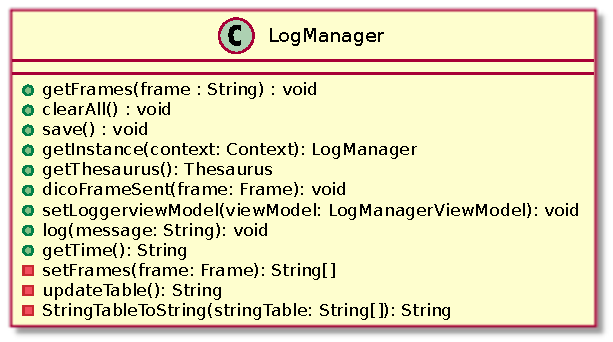
\includegraphics[width=0.80\linewidth]{../schemas/Conception_detaillee/classe_LogManager.pdf}
    \captionof{figure}{Diagramme de classe de LogManager}
\end{minipage}

\subparagraph{Philosophie de conception \newline} 

\medspace

La classe LogManager a pour rôle de traiter les trames reçues depuis la classe DispatcherCANdroid. En effet, lorsque la trame est reçue, elle doit être analysée pour savoir si elle a été envoyée ou non. De plus, elle est mise en forme afin de correspondre à l'affichage. 

\subparagraph{Description structurelle \newline}

\medspace

\textbf{Attributs :}

N.A.

\textbf{Services offerts :}

\begin{itemize}
    \item \textbf{dicoFrameSent(frame : Frame ) : void} --- Opération qui ajoute au dictionnaire la trame envoyée. 
    \item \textbf{setFrame(frame : String ) : String } --- Opération qui met en forme la trame pour l'afficher.
    \item \textbf{getFrames(frame : String ) : void } --- Opération qui récupère les trames reçues. 
    \item \textbf{clearAll() : void } --- Opération qui permet de vider le sniffer en faisant appel à logManagerViewModel. 
    \item \textbf{save() : void } --- Opération qui permet de sauvegarder le fichier en cours.  
    \item \textbf{getInstance(context: Context): LogManager} --- Opération qui permet de retourner une instance de la classe. 
    \item \textbf{getThesaurus(): Thesaurus} --- Opération qui permet de retourner le dictionnaire. 
    \item \textbf{dicoFrameSent(frame: Frame): void} --- Opération qui ajoute au dictionnaire la trame envoyée. 
    \item \textbf{setLoggerviewModel(viewModel: LogManagerViewModel): void} --- Opération qui permet de définir le viewModel. 
    \item \textbf{log(message: String): void} --- Opération qui permet de transmettre le message au viewModel. 
    \item \textbf{getTime(): String} --- Opération qui permet de retourner l'heure. 
    \item \textbf{setFrames(frame: Frame): String[]} --- Opération qui met en forme la trame pour l'afficher. 
    \item \textbf{updateTable(): String} --- Opération qui permet de mettre à jour le tableau comme souhaité pour l'affichage. 
    \item \textbf{StringTableToString(stringTable: String[]): String} --- Opération qui permet de transformer le tableau de String en String.
\end{itemize}